\chapter{基于用户定位的广告投放服务系统架构}
\label{cha:sys_arch}

\section{总体系统结构}

\begin{figure}[tb]
	\centering
	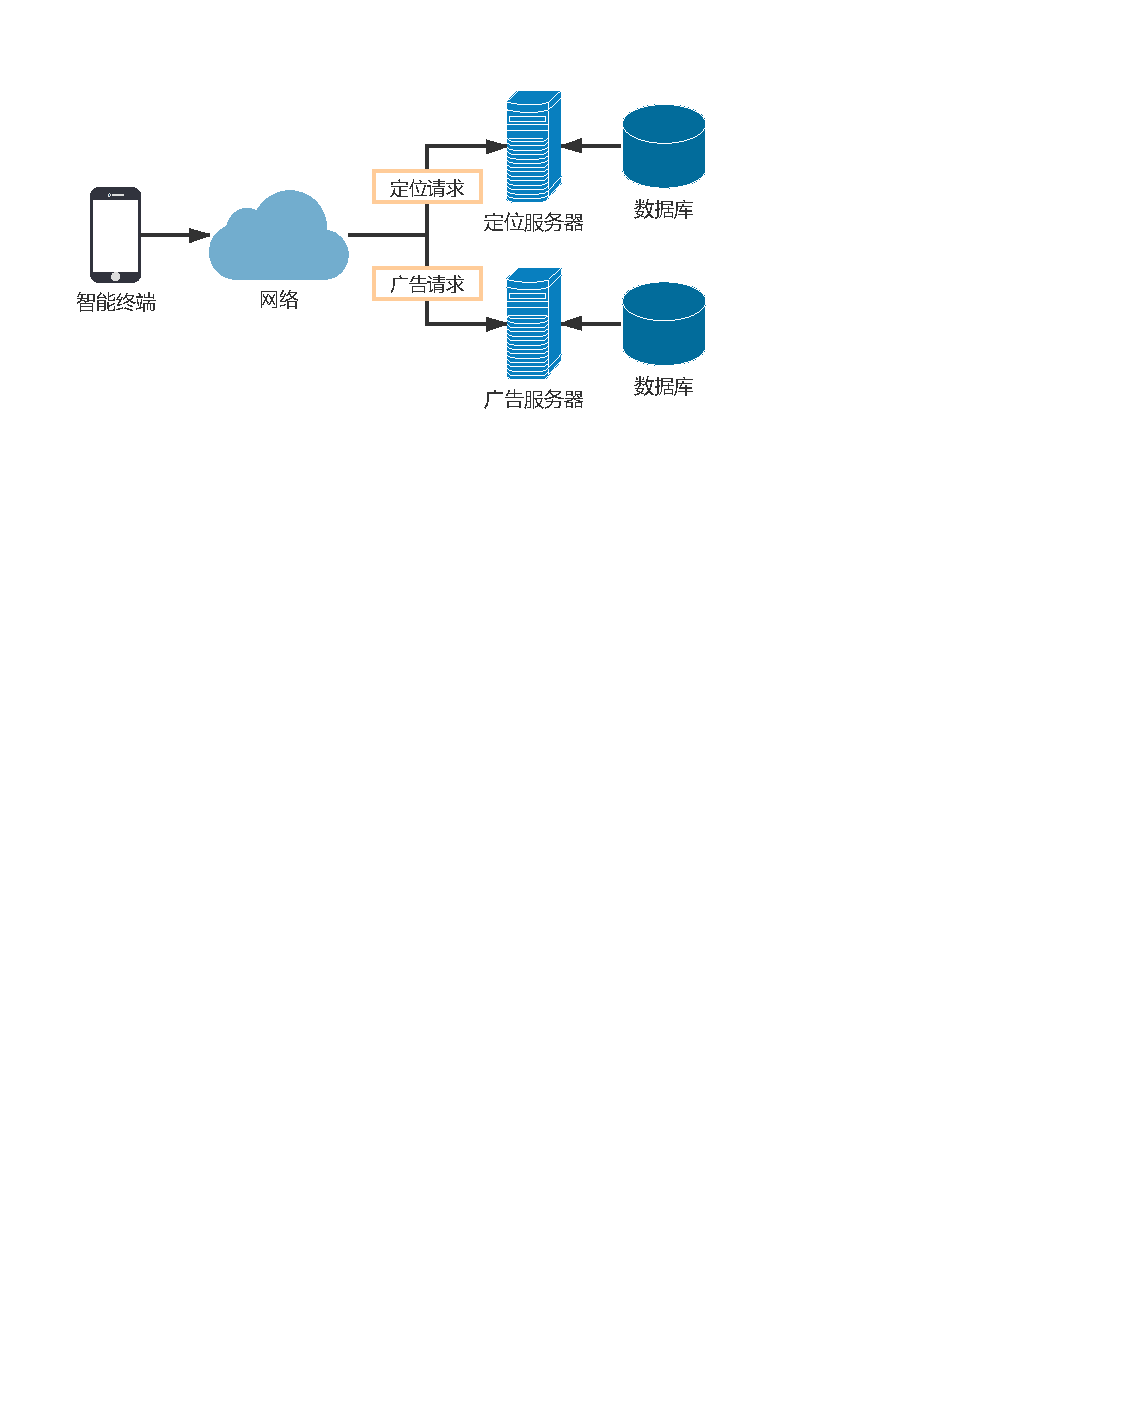
\includegraphics[width=\textwidth]{sys_arch.pdf}
	\caption{如图所示为整个服务机制的系统架构图。智能终端会先向定位服务器发送定位请求,定位服务器根据用户是信号发射源或接收端采取不同的算法计算用户位置,之后返回给终端。获得位置后,终端将向广告服务器发送广告请求,服务器计算完成后返回要投放给用户的广告。}
	\label{fig:sysarch}
\end{figure}

图\ref{fig:sysarch}所示为基于用户定位的广告投放系统总体框架。该系统由两大模块构成:定位服务模块和广告服务模块。每次用户访问该系统时,首先获取自己的定位信息,之后连同自己的位置信息发起广告请求,广告服务器经过计算返回所投放的广告。
\begin{itemize}
	\item 在定位模块中,如果终端是信号发射源,则数据库中存储着WAP接收到的该终端的RSS;若终端是信号接收端,则数据库中存储着历史上不同位置的RSS。从数据库中提取的数据被发送到定位服务器计算定位,最后位置被返回给终端。
	\item 在广告模块中,广告服务器其实是广告服务器群,因为这一部分由多个子模块组成,下一小节将详细介绍其系统架构和模块功能。数据库存储着广告的具体内容,即视频、图片或文本形式的广告内容,在广告服务器决定要投放的广告之后到数据库提取相应的广告内容,并推送给用户。
\end{itemize}

当然图\ref{fig:sysarch}所展示的结构只是多种可能实现中的一种,比如定位信息的获取不是必须从定位服务器获取,也可以是在终端本地计算获得(比如卫星定位),只不过本文所提出的两种定位算法均需要在服务器计算获得定位信息。

\section{广告服务器系统架构}

\begin{figure}[tb]
	\centering
	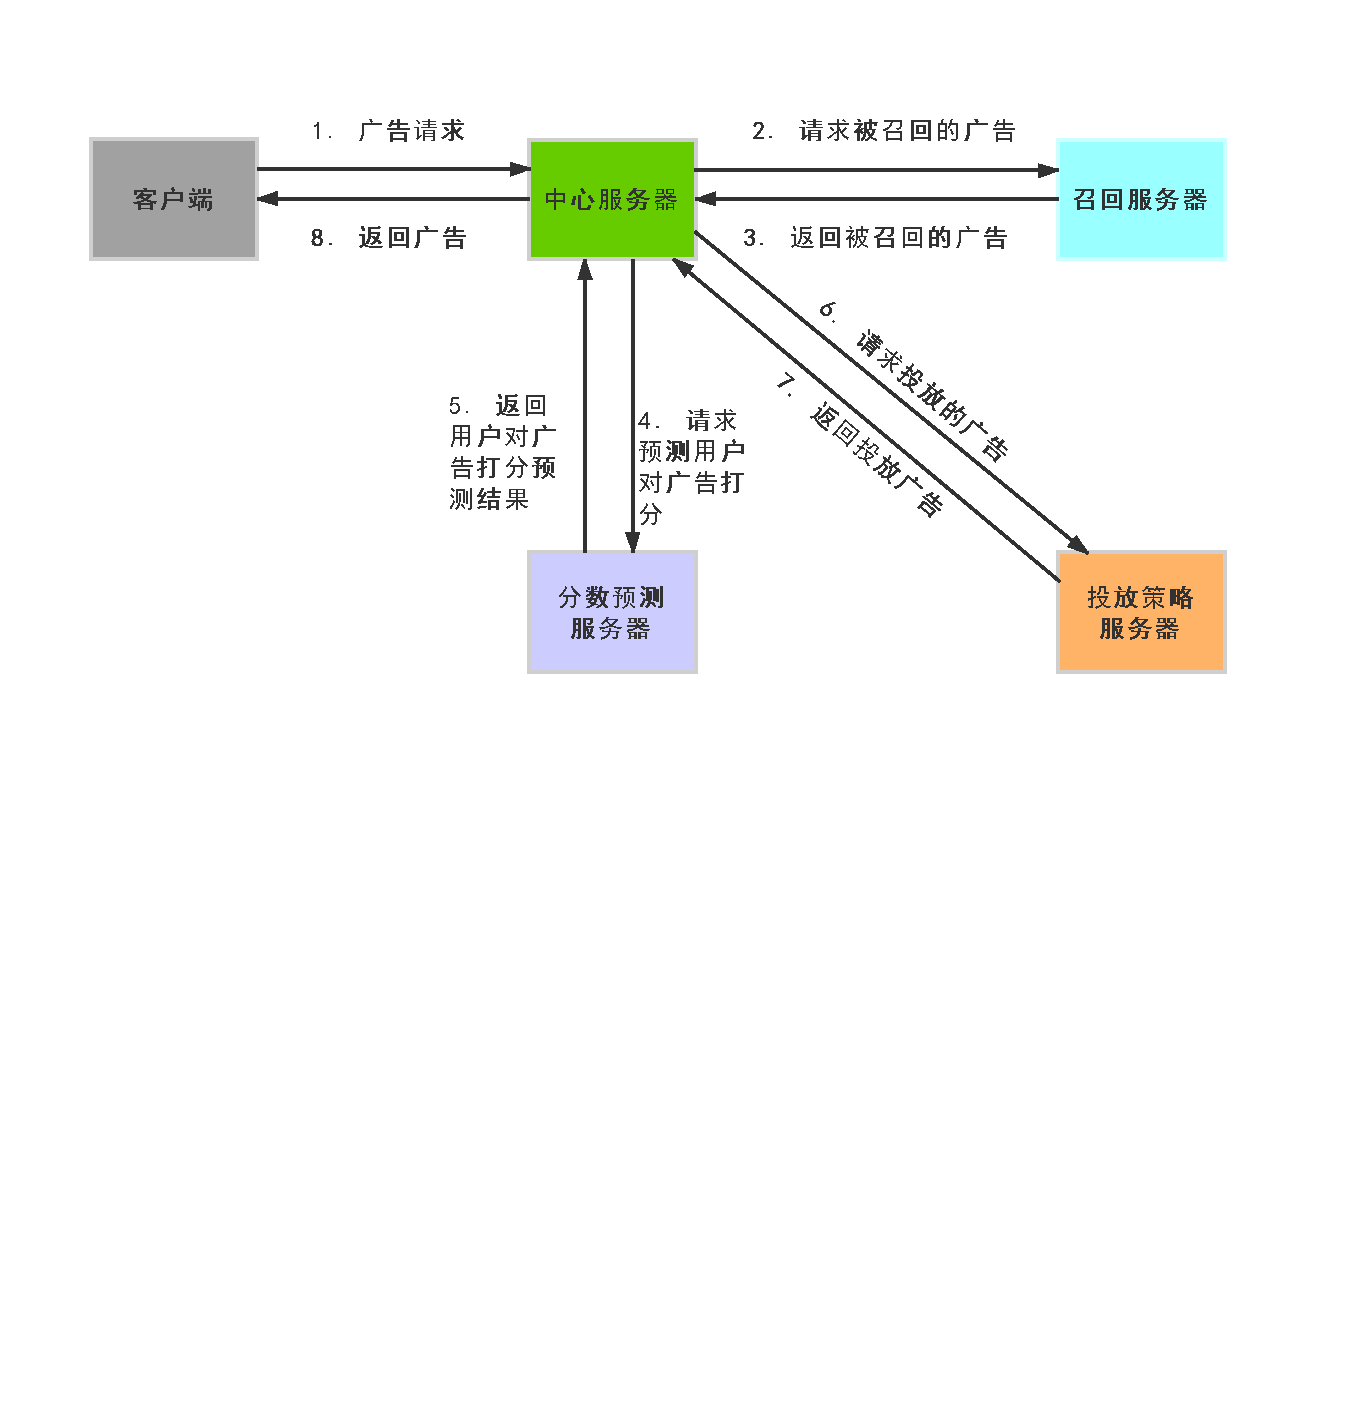
\includegraphics[width=\textwidth]{FansTop_process_cn.pdf}
	\caption{如图所示为针对一次访问投放广告的工作流程,其中箭头上的序号代表了执行顺序。流程从客户端发起广告请求开始,之后中心服务器依次请求召回广、预测用户对被召回广告的打分和打算投放的广告。我们的算法将部署在投放策略服务器上。中心服务器、召回服务器、分数预测服务器和投放策略服务器共同构成了广告服务器(群)。}
	\label{fig:fssys}
\end{figure}

广告服务器(群)的具体结构如图\ref{fig:fssys}所示。每次客户端发起广告请求,广告服务器将按照如下四步执行操作:
\begin{enumerate}
	\item 召回。因为广告数量与服务器计算能力之间的矛盾,只有部分广告会参与后续流程,这个粗略过滤的操作被称作“召回”(Retrieval)或“候选集生成”(Candidate Generation)。因为我们的算法要部署在同城页,这里仅介绍同城页的召回策略,即候选广告是根据访问用户与广告主之间的距离筛选的,这里需要用到上文的定位信息;
	\item 分数预测。在召回广告返回后,中心服务器会向分数预测服务器发送请求预测这些广告的用户打分。预测服务器会根据广告特征、用户特征和过往行为数据对当前广告预测分数。更详细的,预测服务器会返回CTR和FTR的线性组合:
	\begin{equation}
		score = CTR \times  (b + a \times FTR), \label{eq:score}
	\end{equation}
	其中 $a$ 和 $b$ 是线性组合系数。需要注意,这里的FTR是条件概率,即在用户点击广告的条件下,用户关注的概率;
	\item 投放广告,这也是第\ref{cha:allocation}章主要描述的部分。中心服务器在向投放策略服务器请求要投放的广告的同时,也会把召回的广告及其分数一起发送。计算完成后返回给中心服务器决定投放的广告。我们的算法和之前部署的流控算法唯一区别就在投放策略服务器上;
	\item 获取广告内容后,中心服务器将广告返回客户端。
\end{enumerate}

上述流程和框图是广告服务器的大致框架。限于篇幅原因,其他一些与算法无关的底层实现将不会在这里讨论。





